\chapter{Icecube Neutrino Observatory}

Why is icecube so big, bit science smalltalk here?
The IceCube Neutrino observatory is the largest neutrino detector on earth.
Located on the south pole and shown schematically in figure \ref{fig:icecube}.

\begin{figure}
    \centering
    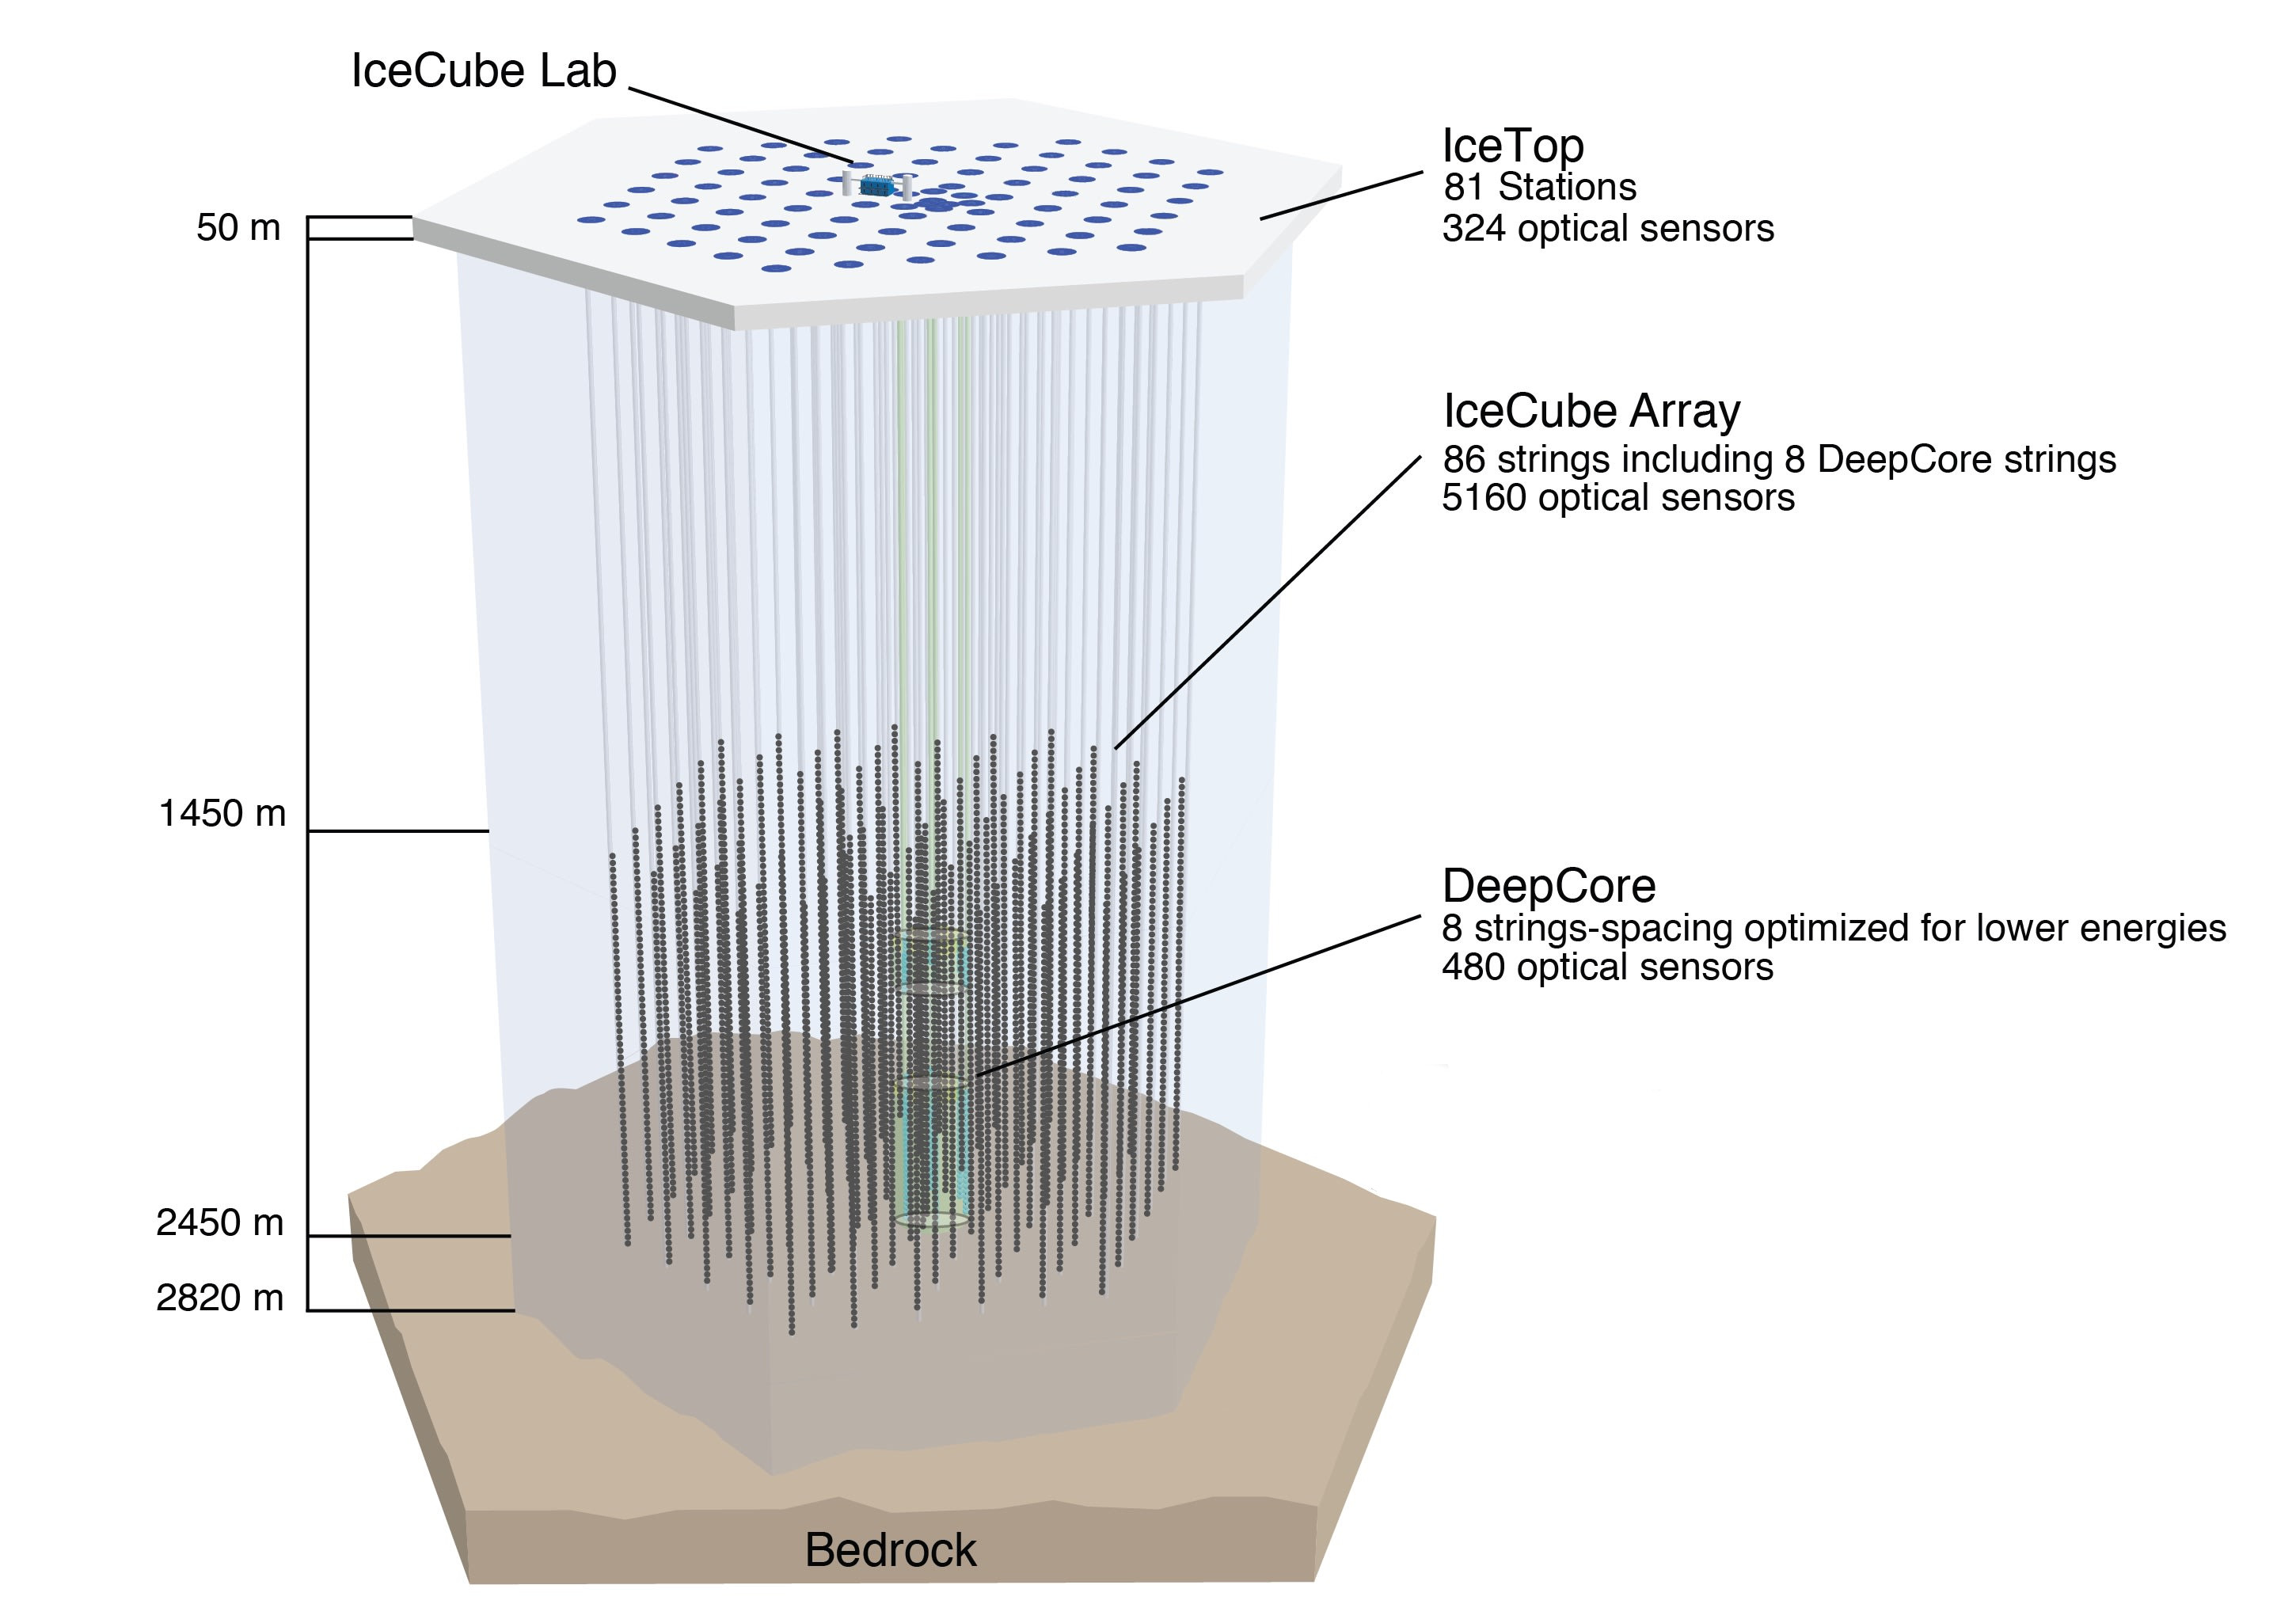
\includegraphics[width=10cm]{Plots/01_7_icecube/IceCube-Array.jpg}
    \caption{\cite{icecube_wesite}.}
    \label{fig:icecube}
\end{figure}

Construction started 2004 and took 7 years to its completion in 2010.
The detector volume of IceCube covers about 1 cubic kilometer of clear antarctic ice.
86 holes were drilled in the ice to let down cables with 60 digital optical modules (DOMs) each.
The detecion volume, or the position of the first DOM respectively, starts at a depth of about 1450 meters and ends in a depth of about 2450 meters.
Mention IceTop and DeepCore?
IceCube detects about 275 million cosmic rays every day.
bit more about doms


\section{Detection Principle}
cherenkov something something\\
show interaction\\
make a figure to cherenkov\\

\section{Tracks and Cascades}
show side by side cascades and tracks\\
what is good about tracks:\\
good angular reconstruction\\
what is good about cascades:\\
high energy, good energy reconstruction\\
